% SEA submission in the LIPIcs style. Built by `make sea` (build/sea/sea.pdf). The body is kept in step with
% ../short/short.tex. \anontrue for the anonymized submission, \anonfalse for the camera-ready version.
\documentclass[a4paper,USenglish,cleveref,anonymous]{lipics-v2021}

\usepackage{cancel}
\usepackage{booktabs}
\usepackage{array}
\usepackage{siunitx}
\usepackage{tikz}
\usepackage{float}
\usepackage{algorithm}
\usepackage[noend]{algpseudocode}

\sisetup{detect-all, exponent-product=\times}
\let\origtextsc\textsc
\renewcommand{\textsc}[1]{\textup{\origtextsc{#1}}}

% anonymization: self-citations (the tdoku NEON port, the full version) and the repository link are hidden
\newif\ifanon
\anontrue
\newcommand{\selfcite}[1]{\ifanon[anonymized]\else\cite{#1}\fi}

\bibliographystyle{plainurl}

\title{Fewer, Better Guesses: A Scalar Band Solver, and When It Beats SIMD Sudoku Solvers}
\titlerunning{A Scalar Band Solver, and When It Beats SIMD Sudoku Solvers}

\author{James Kelly}{Independent researcher, USA}{}{}{}
\authorrunning{J. Kelly}
\Copyright{James Kelly}

\ccsdesc[500]{Theory of computation~Design and analysis of algorithms}
\ccsdesc[300]{Computing methodologies~Search methodologies}

\keywords{Sudoku, constraint propagation, perfect matching, branching heuristics, bit-parallel algorithms, SIMD,
algorithm engineering}

\relatedversion{}
\acknowledgements{FastBandSolver's representation follows zhouyundong's band solver and its implementations
in JCZSolve and rust\_sudoku; the benchmark harness and data sets are Tom Dillon's.}

\nolinenumbers

%Editor-only macros:: begin (do not touch as author)%%%%%%%%%%%%%%%%%%%%%%%%%%%%%%%%%%
\EventEditors{John Q. Open and Joan R. Access}
\EventNoEds{2}
\EventLongTitle{25th International Symposium on Experimental Algorithms (SEA 2027)}
\EventShortTitle{SEA 2027}
\EventAcronym{SEA}
\EventYear{2027}
\EventDate{}
\EventLocation{}
\EventLogo{}
\SeriesVolume{}
\ArticleNo{}
%%%%%%%%%%%%%%%%%%%%%%%%%%%%%%%%%%%%%%%%%%%%%%%%%%%%%%

\begin{document}

\maketitle

\begin{abstract}
The fastest published solver for hard Sudoku puzzles, tdoku, encodes the grid in SIMD registers. We show that a
scalar solver can match or beat it, and explain when. FastBandSolver builds on the band representation of
zhouyundong and JCZSolve, which stores each digit's candidates in a band of three boxes as a 27-bit mask, and makes
three changes: a \emph{stack rule} that applies Simonis's matching constraint between bands and columns with one table
lookup, branching on the two-candidate cell with the most unsolved peers, and a fewest-candidates fallback. On an
Apple M4 Max, checking uniqueness as tdoku's benchmarks do, it is 1.07--1.62$\times$ faster than tdoku (ported to ARM
NEON) on all five of tdoku's standard data sets, and 1.17$\times$ faster on the hardest; an ablation attributes most of
the gain to branching, with 138 guesses per puzzle on that set where JCZSolve makes 363. On x86 the outcome depends on
the processor: FastBandSolver is level or faster on AMD Zen~3, 4--8\% slower on Zen~4, and about 0.7 times tdoku's
speed on Intel. Hardware counters separate three causes: the instruction set (tdoku needs 1.29 times FastBandSolver's
instructions on NEON but 0.60--0.67 times on x86), the core (on the same x86 binary, Intel cores run tdoku's code
faster per cycle than AMD's), and AVX-512, which saves tdoku another 12\% of its cycles on Intel.
\end{abstract}

\section{Introduction}
\label{sec:intro}

Solving a single Sudoku is easy for a computer, but solving and \emph{proving uniqueness} of millions of hard
puzzles quickly matters to puzzle generators, to difficulty raters and to exhaustive searches such as the proof
that no 16-clue Sudoku exists~\cite{mcguire2014sixteen}. Deciding whether such a puzzle has another solution is
NP-complete~\cite{yato2003complexity}, so every fast solver is a search with propagation, and the design space is the
classic one of constraint programming~\cite{simonis2005sudoku} and SAT~\cite{lynce2006sudoku}: how much inference to do
at each node, and where to branch.

The current reference point is tdoku~\cite{dillon2019tdoku,dillon2019nerdsniped}. It encodes the grid in 128- or
256-bit SIMD registers (single instruction, multiple data: one instruction operates on several small values held side
by side in a wide register) and propagates strongly, and in its author's benchmark it is well ahead of the other fast
solvers on hard puzzles. tdoku is written for x86 SIMD; to compare it on ARM we added native NEON support to
it~\selfcite{kelly2026tdokuarm}.

This paper asks whether a \emph{scalar} solver, one that uses only ordinary 32- and 64-bit integer instructions and no SIMD, can beat tdoku on hard puzzles, and on which processors. Our contributions:
\begin{itemize}
\item \textbf{FastBandSolver}, an open-source scalar C++ solver (\cref{sec:solver}). It extends the band solvers
  zhouyundong and JCZSolve with a \textbf{stack rule} (\cref{sec:rules}): within each column of three boxes, each digit's
  placements pair the three bands one-to-one with the three columns, and any (band, column) choice that fits no such
  pairing is removed. The constraint is Simonis's~\cite{simonis2005sudoku}; we apply it with one table lookup, only when
  a band's columns change.
\item \textbf{Better branching}: the two-candidate cell with the most unsolved peers instead of the first one found,
  and a fewest-candidates fallback when no cell has two candidates. An ablation (\cref{tab:ablation}) shows that
  branching, not propagation, carries most of the gain.
\item \textbf{Results on the M4} (\cref{sec:results}): FastBandSolver is faster than native tdoku on all five of
  tdoku's standard data sets, both when checking uniqueness and when one solution is enough.
\item \textbf{When it wins on x86, and why} (\cref{sec:x86}): measured on seven x86 cloud machines, the outcome depends
  on the processor, and hardware counters on ten processors separate the instruction set, the core and AVX-512 as
  causes.
\end{itemize}
A full version of this paper~\selfcite{kelly2026full} proves that the rules are sound and that the solver counts solutions
exactly, describes a parallel version that solves the hardest puzzles $2.1\times$ faster on 4 threads, and reports six
approaches that did not beat tdoku, with measurements. The code is open source.\footnote{\ifanon\textbf{[anonymized repository URL]}\else\textbf{[repository URL]}\fi}

% ---------------------------------------------------------------- to be written, one section at a time
\section{Background and related work}
\label{sec:related}

\subparagraph{Terms.} A grid has 81 cells in 9 rows, 9 columns and 9 boxes; rows, columns and boxes are \emph{units},
and the \emph{peers} of a cell are the 20 other cells that share a unit with it. A \emph{band} is a horizontal strip of
three boxes and a \emph{stack} a vertical one; each box is where one band and one stack cross. Within a band, the three
cells where a row crosses a box form a \emph{triad}~\cite{dillon2019nerdsniped}. A solver keeps each cell's
\emph{candidates}, the digits that can still go there, and alternates \emph{propagation}, which removes candidates by
rules, with \emph{search}, which guesses when the rules run out. The cheap rules are the \emph{naked single} (a cell
with one candidate), the \emph{hidden single} (a digit with one place left in a unit) and \emph{locked candidates}
(a digit confined to the overlap of a box with a row or column). Following tdoku's benchmark, every solver here is
asked for up to two solutions (a \emph{solution limit} of 2), so on a well-formed puzzle it must search the whole tree
to prove uniqueness, and the time is roughly the number of nodes times the time per node. We count one \emph{guess}
per two-candidate branch and $n-1$ for a cell with $n$ candidates.

\subparagraph{Band solvers.} zhouyundong's solver~\cite{zhouyundong2012solver}, refined by champagne and JasonLion into
JCZSolve~\cite{jczsolve2016} and ported to Rust as rust\_sudoku~\cite{emerentius2018sudoku}, stores one 32-bit word per
(digit, band) whose 27 low bits mark the cells of the band where the digit can still go. For each word that changed,
its update compresses each row into the boxes the digit can still use, keeps only the parts of that $3\times 3$
row-by-box pattern that some assignment of rows to boxes can use (zero means a contradiction), removes locked columns
from the other bands, and places rows that are down to one cell, all with 512-entry lookup tables. It then counts, for
all 27 cells of a band at once, how many digits each cell admits, with three words meaning ``at least one'', ``at least
two'' and ``at least three'', places naked singles, and guesses on the first two-candidate cell in board order, or on
the first unsolved cell if there is none. FastBandSolver starts from this design.

\subparagraph{tdoku.} Dillon's tdoku~\cite{dillon2019tdoku,dillon2019nerdsniped} starts from a SAT encoding, adds
variables for horizontal and vertical triads so that locked candidates follow from cardinality constraints, and keeps,
for each band and stack and each of its six \emph{configurations} (the six ways to assign its rows to its boxes, or its
columns to its boxes), the digits that can still take it; this is our band rule in another form, kept for rows and
columns alike. Each box is one 256-bit register of sixteen 16-bit lanes, and propagation is branch-free message passing
between boxes and bands. It branches on a configuration of the band with the fewest remaining configurations. In its
author's benchmark on an Intel i5-8600k at limit 2, it is about 1.5 times the geometric mean speed of the other solvers
on magictour and nearly twice on the hardest set.

\subparagraph{Matchings.} A \emph{perfect matching} of a bipartite graph is a set of edges that uses every vertex exactly
once; with three vertices on each side it is one of the $3!=6$ one-to-one pairings whose three pairs are all edges, and
an edge on no perfect matching can be deleted when every vertex must be matched. R\'egin's
algorithm~\cite{regin1994filtering} deletes all such edges for \texttt{alldifferent} constraints, and
Simonis~\cite{simonis2005sudoku} used it for Sudoku, adding redundant constraints for the interactions between units.
One of them (his Section 5.3) is a matching between the rows of a band and its boxes for each digit, with its
counterpart for columns and boxes; these are our band and stack rules. He solves them with a general matching
algorithm; we precompute every $3\times 3$ case in a 512-entry table.

\subparagraph{Branching.} Choosing the variable with the fewest remaining values~\cite{haralick1980increasing} is the
classic heuristic; band solvers use the cheaper ``first two-candidate cell''. Breaking ties by the number of unassigned
neighbours, the \emph{degree} heuristic, goes back to Br\'elaz's DSATUR~\cite{brelaz1979new}, and has been evaluated on
Sudoku in generic constraint solvers~\cite{bakker2015generic,liu2026dibs} but not, as far as we know, in a fast solver.

\subparagraph{Recent solvers.} fastdoku~\cite{rocketbombs2026fastdoku} chooses per puzzle between a JCZSolve-style band
engine and a reimplementation of tdoku's, and reports 1.06--1.63 times the speed of the faster of tdoku and
rust\_sudoku on x86, timing the \emph{first} solution; its band engine branches on the first two-candidate cell.
RKCR7~\cite{rkcr7_2026autoresearch} reports beating tdoku on four of six data sets, but its own solver stops at the
first solution while tdoku was timed at limit 2. Searching GitHub, the Sudoku Players' Forum, arXiv and the
constraint-programming literature in September 2026, we found no earlier solver that beats tdoku at limit 2, and no
fast band solver that uses the stack rule or the degree tie-break.

\section{The band and stack rules}
\label{sec:rules}

\subparagraph{The idea in plain terms.} Look at one digit, say 5, in one band. The finished grid will have exactly one 5
in each of the band's three rows and exactly one in each of its three boxes. So the three 5s pair the rows with the
boxes: each row gets its own box. Some pairings may already be impossible because 5 has been ruled out of that part of
the row. If a particular row--box combination cannot be part of \emph{any} complete pairing, then 5 cannot go in that
triad, even though nothing in the triad itself rules it out. This one idea, checked with a lookup table,
covers locked candidates between rows and boxes, and it narrows a box that has a single place left for the digit down
to a row with a single place left, which the solver then fills. The \emph{band rule} is this check. In the terms of
\cref{sec:related}, the band's rows and boxes are the two sides of a bipartite graph, row $r$ is joined to box $k$ when
the digit can still go in their triad, the digit's three placements form a perfect matching, and every edge that lies
on no perfect matching is deleted. \Cref{fig:band} works through an example. The rule removes whole triads; it never
chooses between the cells of one.

\begin{figure}[tbp]
\centering
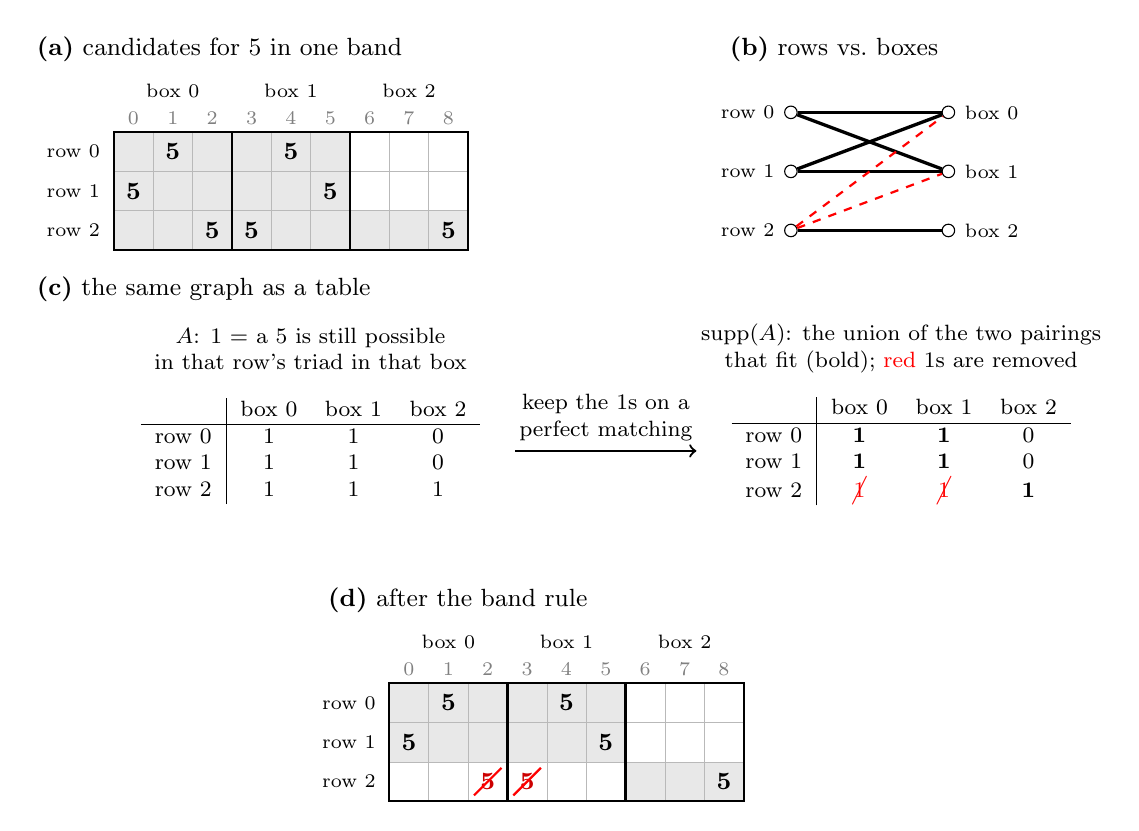
\begin{tikzpicture}[x=0.5cm,y=0.5cm,
  cand/.style={font=\small\bfseries},
  gone/.style={font=\small\bfseries,red!80!black},
  vtx/.style={circle,draw,fill=white,inner sep=1.6pt}]
  % ---------- (a) before ----------
  \begin{scope}
    \node[anchor=west] at (-2.2,5.1) {\small\textbf{(a)} candidates for 5 in one band};
    \foreach \r/\k in {0/0,0/1,1/0,1/1,2/0,2/1,2/2} \fill[gray!18] (3*\k,2-\r) rectangle (3*\k+3,3-\r);
    \draw[step=1,gray!55,very thin] (0,0) grid (9,3);
    \draw[thick] (0,0) rectangle (9,3);
    \foreach \x in {3,6} \draw[thick] (\x,0) -- (\x,3);
    \foreach \c in {0,...,8} \node[font=\scriptsize,gray] at (\c+0.5,3.35) {\c};
    \foreach \k in {0,1,2} \node[font=\scriptsize] at (3*\k+1.5,4.05) {box \k};
    \foreach \r in {0,1,2} \node[font=\scriptsize,anchor=east] at (-0.1,2.5-\r) {row \r};
    \foreach \r/\c in {0/1,0/4,1/0,1/5,2/2,2/3,2/8} \node[cand] at (\c+0.5,2.5-\r) {5};
  \end{scope}
  % ---------- (b) graph ----------
  \begin{scope}[xshift=8.6cm]
    \node[anchor=west] at (-1.8,5.1) {\small\textbf{(b)} rows vs.\ boxes};
    \foreach \r in {0,1,2} \node[vtx,label={[font=\scriptsize]left:row \r}] (r\r) at (0,3.5-1.5*\r) {};
    \foreach \k in {0,1,2} \node[vtx,label={[font=\scriptsize]right:box \k}] (b\k) at (4,3.5-1.5*\k) {};
    \draw[very thick] (r0) -- (b0);
    \draw[very thick] (r0) -- (b1);
    \draw[very thick] (r1) -- (b0);
    \draw[very thick] (r1) -- (b1);
    \draw[very thick] (r2) -- (b2);
    \draw[dashed,thick,red] (r2) -- (b0);
    \draw[dashed,thick,red] (r2) -- (b1);
  \end{scope}
  % ---------- (c) matrices ----------
  \begin{scope}[yshift=-3.3cm]
    \node[anchor=west] at (-2.2,5.6) {\small\textbf{(c)} the same graph as a table};
    \node[font=\footnotesize,align=center] at (5.0,4.1) {$A$: 1 = a 5 is still possible\\ in that row's triad in that box};
    \node[font=\footnotesize] at (5.0,1.5) {$\begin{array}{r|ccc}
        & \text{box }0 & \text{box }1 & \text{box }2 \\ \hline
      \text{row }0 & 1 & 1 & 0 \\
      \text{row }1 & 1 & 1 & 0 \\
      \text{row }2 & 1 & 1 & 1
      \end{array}$};
    \draw[->,thick] (10.2,1.5) -- (14.8,1.5) node[midway,above,font=\footnotesize,align=center] {keep the 1s on a\\perfect matching};
    \node[font=\footnotesize,align=center] at (20.0,4.1) {$\mathrm{supp}(A)$: the union of the two pairings\\ that fit (bold); \textcolor{red}{red} 1s are removed};
    \node[font=\footnotesize] at (20.0,1.5) {$\begin{array}{r|ccc}
        & \text{box }0 & \text{box }1 & \text{box }2 \\ \hline
      \text{row }0 & \mathbf{1} & \mathbf{1} & 0 \\
      \text{row }1 & \mathbf{1} & \mathbf{1} & 0 \\
      \text{row }2 & \textcolor{red}{\cancel{1}} & \textcolor{red}{\cancel{1}} & \mathbf{1}
      \end{array}$};
  \end{scope}
  % ---------- (d) after ----------
  \begin{scope}[xshift=3.5cm,yshift=-7.0cm]
    \node[anchor=west] at (-1.8,5.1) {\small\textbf{(d)} after the band rule};
    \foreach \c in {0,...,8} \node[font=\scriptsize,gray] at (\c+0.5,3.35) {\c};
    \foreach \k in {0,1,2} \node[font=\scriptsize] at (3*\k+1.5,4.05) {box \k};
    \foreach \r in {0,1,2} \node[font=\scriptsize,anchor=east] at (-0.1,2.5-\r) {row \r};
    \foreach \r/\k in {0/0,0/1,1/0,1/1,2/2} \fill[gray!18] (3*\k,2-\r) rectangle (3*\k+3,3-\r);
    \draw[step=1,gray!55,very thin] (0,0) grid (9,3);
    \draw[thick] (0,0) rectangle (9,3);
    \foreach \x in {3,6} \draw[thick] (\x,0) -- (\x,3);
    \foreach \r/\c in {0/1,0/4,1/0,1/5,2/8} \node[cand] at (\c+0.5,2.5-\r) {5};
    \foreach \r/\c in {2/2,2/3} {
      \node[gone] at (\c+0.5,2.5-\r) {5};
      \draw[red,thick] (\c+0.15,2.15-\r) -- (\c+0.85,2.85-\r);
    }
  \end{scope}
\end{tikzpicture}
\caption{The band rule for the digit 5, on an example. (a) The band's three rows and three
boxes; 5 is still a candidate in the cells shown, and the shaded triads are those that contain a candidate. (b) The
bipartite graph: an edge joins row $r$ and box $k$ when triad $(r,k)$ is shaded. Rows 0 and 1 are joined only to
boxes 0 and 1, so they use up both, and row 2 must take box 2. Two perfect matchings remain (row 0 with box 0 and row 1
with box 1, or the other way round), and the black edges are their union. The two red dashed edges are in no perfect
matching. (c) The same graph as a table $A$: one row of the table per row of the band, one column per box, and a 1 where the
graph has an edge, that is, where 5 is still possible in that triad. Keeping only the 1s that lie on a perfect
matching gives $\mathrm{supp}(A)$: the bold 1s are the union of the two pairings that fit, and the red 1s, the dashed
edges of (b), are removed. (d) Removing the red edges removes 5 from triads (row 2, box 0) and (row 2, box 1): the
candidates in columns 2 and 3 of row 2 are eliminated, although nothing in their own row, column or box rules them
out directly. The stack rule is the same test with bands in place of rows and a stack's
columns in place of boxes.}
\label{fig:band}
\end{figure}

\subparagraph{The stack rule.} The \emph{stack rule} is the same check turned sideways. In a stack, the digit appears once
in each of the stack's three columns and once in each of its three boxes, and the three boxes of a stack lie in three
different bands, so the digit's three placements pair the bands one-to-one with the stack's columns. The graph has the
three bands on one side and the stack's three columns on the other, with an edge from band $b$ to column $c$ when the
digit can still go in column $c$ within band $b$, and every edge that lies on no perfect matching is deleted: the digit
is removed from that column within that band. For example, if in one stack 5 can go in columns 0 and 1 in band 0, only
in column 0 in band 1, and in any of the three columns in band 2, then band 1 must take column 0, band 0 column 1 and
band 2 column 2, and three of the six edges are deleted. The locked-column step of JCZSolve is the special case of a
band joined to a single column, and tdoku gets the same inference from its vertical triads.

\subparagraph{Soundness.} Both rules remove only candidates that no solution can use. In a solution, a digit occupies
one cell in each row of a band and one in each of its boxes, so the triads that hold it pair the rows one-to-one with
the boxes, using only triads where it was still a candidate: a perfect matching. A triad on no perfect matching
therefore never holds the digit, and if no perfect matching exists the position has no solution. The stack rule is the
same argument with bands and columns. The full version~\selfcite{kelly2026full} proves this, and that the solver built on
these rules counts solutions exactly and terminates.

\subparagraph{Hidden singles.} FastBandSolver looks for hidden singles only in rows. Together with the two rules, that
loses nothing: once propagation stops, in any position that has a solution, a digit with a single place left in a box
or a column also has a single place left in that cell's row, so the row step has already placed it (proved in the full
version). In a reference solver that applies every rule in every round, removing box and column hidden singles leaves
the search tree unchanged on the hardest set (284.2 nodes per puzzle either way).


\section{FastBandSolver}
\label{sec:solver}

FastBandSolver is a single C++20 header of about 400 lines that solves one puzzle at a time on one thread.

\subparagraph{State.} For digit $d\in\{1,\dots,9\}$ and band $b\in\{0,1,2\}$, the 32-bit word $M_{d,b}$ holds a 27-bit
mask of the cells of band $b$ where $d$ can still go, with bit $9r+c$ for row $r\in\{0,1,2\}$ of the band and column
$c\in\{0,\dots,8\}$; bits $9r+3k$ to $9r+3k+2$ are the triad of row $r$ and box $k$. The band's \emph{column set}
$P(M)=(M \mid M\gg 9 \mid M\gg 18)\,\&\,111\,111\,111_2$ marks the columns where the digit still has a candidate, and
$\mathrm{cols}(x)=x \mid x\ll 9 \mid x\ll 18$ spreads a 9-bit column set back to cells. Most of the work is on whole
bands, one instruction per 27-bit word. A search state holds the 27 masks, a copy of each mask as it was when the band
rules last ran on it (\texttt{checked}, 0 at first), a mask of unsolved cells per band, and per digit the rows where
it is not yet placed: 246 bytes. The solver owns an array of 82 states; a guess copies slot $t$ into slot $t+1$ with
one \texttt{memcpy}, and nothing is allocated during a solve. Its lookup tables, 8.5\,KB in all, are computed at
compile time from their definitions.

\begin{algorithm}[t]
\caption{\textsc{UpdateBand}$_b(S, d)$: band rule, stack rule and row singles for digit $d$ in band $b$}
\label{alg:band}
\begin{algorithmic}[1]
\State $\mathit{bandCells} \gets S.\mathit{valueToBand}[d-1][b]$; \ $\mathit{lastChecked} \gets S.\mathit{checked}[d-1][b]$
\State $\mathit{boxCandidates} \gets \textsc{BoxesOfRow}[\mathit{bandCells} \,\&\, 111\,111\,111_2]$
  \Statex \hspace{\algorithmicindent}\hspace{\algorithmicindent}$\mid \textsc{BoxesOfRow}[(\mathit{bandCells}\gg 9)\,\&\,111\,111\,111_2]\ll 3$
  \Statex \hspace{\algorithmicindent}\hspace{\algorithmicindent}$\mid \textsc{BoxesOfRow}[\mathit{bandCells}\gg 18]\ll 6$ \Comment{the $3\times 3$ matrix $A^{d,b}$}
\State $\mathit{bandCells} \gets \mathit{bandCells} \,\&\, \textsc{PossibleCells}[\mathit{boxCandidates}]$ \Comment{band rule}
\If{$\mathit{bandCells} = 0$} \Return \textbf{contradiction} \EndIf
\State $S.\mathit{valueToBand}[d-1][b] \gets \mathit{bandCells}$; \ $S.\mathit{checked}[d-1][b] \gets \mathit{bandCells}$
\State $\mathit{columns} \gets \mathrm{bandColumns}(\mathit{bandCells})$
\If{$\mathit{columns} \ne \mathrm{bandColumns}(\mathit{lastChecked})$} \textsc{StackRule}$(S, d)$ \EndIf
\State $\mathit{singleRows} \gets \textsc{SingleRows}[\textsc{PermutationUnion}[\mathit{boxCandidates}]$
  \Statex \hspace{\algorithmicindent}\hspace{\algorithmicindent}$\mid \textsc{OneColumnBoxes}[\mathit{columns}]\ll 9]$
\State $\mathit{openRowsInBand} \gets (S.\mathit{openRows}[d-1] \gg 3b) \,\&\, 111_2$ \Comment{rows where $d$ is not placed yet}
  \Statex \hspace{\algorithmicindent}$\mathit{newSingleRows} \gets \mathit{singleRows} \,\&\, \mathit{openRowsInBand}$
\If{$\mathit{newSingleRows} \ne 0$}
  \State $\mathit{placedCells} \gets \mathit{bandCells} \,\&\, \textsc{RowsCells}[\mathit{newSingleRows}]$ \Comment{one cell per new single row}
  \State $\mathit{digitMaskNow} \gets S.\mathit{valueToBand}[d-1][b]$ \Comment{as left by the stack rule}
  \For{$\mathit{other} \gets 0$ \textbf{to} $8$} $S.\mathit{valueToBand}[\mathit{other}][b] \gets S.\mathit{valueToBand}[\mathit{other}][b] \,\&\, \lnot\mathit{placedCells}$ \EndFor
  \State $S.\mathit{valueToBand}[d-1][b] \gets \mathit{digitMaskNow}$ \Comment{give $d$ its mask back}
  \State $S.\mathit{unsolved}[b] \gets S.\mathit{unsolved}[b] \,\&\, \lnot\mathit{placedCells}$
  \Statex \hspace{\algorithmicindent}$S.\mathit{openRows}[d-1] \gets S.\mathit{openRows}[d-1] \,\&\, \lnot(\mathit{newSingleRows}\ll 3b)$
\EndIf
\State \Return \textbf{ok}
\end{algorithmic}
\end{algorithm}

\subparagraph{The band update.} \Cref{alg:band} runs on one (digit, band) mask. Line 2 turns the mask into the $3\times 3$
row-by-box matrix of \cref{fig:band} with three 512-entry lookups, one per row, and line 3 applies the band rule:
\textsc{PossibleCells}$[\mathit{boxCandidates}]$ holds the cells of the triads on some perfect matching, so one AND
removes every candidate the rule removes, and a zero result is a contradiction (line 4). Line 7 runs the stack rule only
when the band's column set has changed since it was last checked; as \texttt{checked} starts at 0, every band triggers
it on its first update. Line 8 finds the rows that are down to one cell with one 4096-entry lookup: after the band
rule, a row has exactly one cell left exactly when its row of the matching union has a single box and that box has a
single column in the band. Lines 10--15 place those rows' cells, clearing them from all nine digits in straight-line
code and then giving $d$ back its mask as the stack rule left it. The code is a template on the band index, so each of
the three copies has the positions of the other bands as constants, and it is forced inline.

\subparagraph{The stack rule.} For each stack, \textsc{StackRule}$(S,d)$ builds the $3\times 3$ matrix of bands against
the stack's columns from the three column sets $P(M_{d,b})$, looks up \textsc{PermutationUnion}, and keeps each band's
columns on some perfect matching; each mask is then ANDed with $\mathrm{cols}$ of its kept columns. It is branch-free:
three lookups and a few dozen shifts, ANDs and ORs. Processing only the stacks whose columns changed gave the same tree
but was 19\% slower, because the extra branches mispredict.

\subparagraph{Propagation.} \textsc{Update} runs \textsc{UpdateBand} on every mask that differs from its checked copy,
pass after pass, until a pass runs none. \textsc{Propagate} then counts, for each band, how many digits each cell
admits, with three bit-sliced counters updated for each digit $d$ in turn:
\[
\mathit{thrice} \mathrel{|}= \mathit{twice}\,\&\,M_{d,b}, \qquad
\mathit{twice} \mathrel{|}= \mathit{once}\,\&\,M_{d,b}, \qquad
\mathit{once} \mathrel{|}= M_{d,b},
\]
so bit $x$ of each is set when at least one, two or three digits admit cell $x$, for all 27 cells at once. A cell
missing from $\mathit{once}$ is a contradiction; the unsolved cells in $\mathit{once}\,\&\,\lnot\mathit{twice}$ are
naked singles, placed by ANDing the digit's mask with a table entry that removes it from the rest of the cell's row and
box, and its other two masks with one that removes the cell's column; and $\mathit{twice}\,\&\,\lnot\mathit{thrice}$
are the cells with exactly two candidates. If a single was placed, \textsc{Propagate} repeats; otherwise it returns
\emph{solved} when no cell has two or more candidates, and \emph{open} with the two-candidate cells.

\subparagraph{Search.} The search is depth first and stops once \emph{limit} solutions are found. At an open node it takes
the two-candidate cell with the most unsolved peers, the first in board order among ties. For cell $x$ at bit $i$ of
band $b$, the score is
\[
\mathrm{popcount}\bigl(U_b \,\&\, \textsc{BandPeers}[i]\bigr) + \mathrm{popcount}\bigl((U_{b'} \,\&\, \mathrm{col}_i) \mid
(U_{b''} \,\&\, \mathrm{col}_i)\ll 32\bigr),
\]
where $U$ are the unsolved masks, $b'$ and $b''$ the other two bands, \textsc{BandPeers}$[i]$ the cell's row and box
within its band, and $\mathrm{col}_i$ the three cells of its column in a band; packing the two other bands into one
64-bit word makes it two popcounts. The first digit is tried in a copy in slot $t+1$, and the second in slot $t$
itself, which is not needed afterwards. If no cell has two candidates, the fallback takes the unsolved cell with the
fewest candidates, breaking ties by the same score, and tries each candidate in a copy. Placing a digit removes the
cell from the other eight digits' masks and the digit from the cell's peers.

\subparagraph{Correctness and testing.} The full version~\selfcite{kelly2026full} proves that \textsc{Propagate} keeps exactly
the solutions of the node, that a \emph{solved} node is a valid grid, and that the search counts $\min(\mathit{limit},
n)$ solutions in at most 82 states. The proofs rely on masks only ever shrinking, and writing them exposed a bug that no
test had caught: the row-single step once restored $d$'s mask as the band rule had left it, putting back candidates the
stack rule had just removed, about 21 times per puzzle on the hardest set; the solver still agreed with tdoku
everywhere, because the stack rule usually removed them again. We compare solution counts at limits 1, 2 and 3 with
tdoku on all seven of tdoku's data sets, 709{,}764 puzzles including 10{,}000 with several solutions and 486{,}451 with
none, and validate every solution found.

\section{Results}
\label{sec:results}

\subparagraph{Setup.} All measurements in this section are on an Apple M4 Max, macOS 15.6, Apple clang 17.0.0 with
\texttt{-O3 -march=native}, single-threaded. We use tdoku's five standard data sets~\cite{dillon2019nerdsniped}: the
49{,}158 known 17-clue puzzles~\cite{royle17clue,champagne2022all17}, magictour's top
1465~\cite{stertenbrink2005top1465}, the forum-hardest collections (375 puzzles from ``1106'' and 48{,}766 from
``1905\_11+'')~\cite{forumhardest}, and 100{,}000 puzzles from the Kaggle data set~\cite{park2016kaggle}. As in tdoku's
benchmarks, every solver is called with a solution limit of 2 and converting the puzzle string is part of each call;
every solver must solve every puzzle with a valid solution and agree with the others on the number of solutions.
Solvers take turns over the whole data set, and we report the median of seven runs. tdoku is built with our native
NEON port~\selfcite{kelly2026tdokuarm}; JCZSolve, whose source leaves its copyright unspecified, is built from tdoku's copy
for local measurement only. A \texttt{make} target in the repository reproduces \cref{tab:sota} for the other solvers.

\begin{table}[t]
\centering
\caption{Time per puzzle in microseconds (guesses per puzzle in parentheses beneath), limit 2, median of 7 interleaved runs, Apple M4 Max.
Every solver solves every puzzle with a valid solution and agrees on the solution counts. Guesses are each solver's
own count of binary decisions. Between two complete runs of this benchmark on different occasions, every solver's
times moved by up to 3\%, together; ratios between solvers moved by up to 0.03.}
\label{tab:sota}
\small
\setlength{\tabcolsep}{4pt}
\begin{tabular}{lrrrrrr}
\toprule
data set & puzzles & FastBandSolver & tdoku & JCZSolve & jsolve & kudoku \\
\midrule
17 clue & 49158 & \textbf{1.79} & 2.90 & 2.38 & 2.96 & 14.5 \\
&& (0.68) & (0.57) & (2.37) & (0.60) & (4.51) \\[2pt]
magictour top 1465 & 1465 & \textbf{6.90} & 8.31 & 10.0 & 12.8 & 64.2 \\
&& (10.3) & (8.94) & (22.0) & (12.1) & (33.9) \\[2pt]
forum hardest 1106 & 375 & \textbf{62.1} & 72.7 & 107 & 149 & 562 \\
&& (138) & (110) & (363) & (183) & (326) \\[2pt]
forum hardest 1905 11+ & 48766 & \textbf{39.9} & 46.5 & 55.9 & 90.4 & 272 \\
&& (81.0) & (61.7) & (167) & (100) & (142) \\[2pt]
kaggle & 100000 & \textbf{0.864} & 0.922 & 1.17 & 1.55 & 7.48 \\
&& (0) & (0) & (0) & (0) & (0) \\[2pt]
\bottomrule
\end{tabular}
\end{table}

\Cref{tab:sota} compares FastBandSolver with tdoku and with the fastest cell-based (jsolve), band-based (JCZSolve) and
exact-cover (kudoku) solvers from tdoku's benchmark. FastBandSolver is fastest on every set: 1.17$\times$ faster than
tdoku on the 375 hardest puzzles, 1.17$\times$ on the second forum set, 1.20$\times$ on magictour, 1.62$\times$ on
17-clue and 1.07$\times$ on kaggle. tdoku still makes the fewest guesses: its triad propagation and configuration
branching leave a 20\% smaller tree than ours on the hardest set, so FastBandSolver wins on cost per node
(\cref{sec:x86}). With a limit of 1, where a solver stops at the first solution and must write it out,
FastBandSolver is also fastest on all five sets, by 1.07--1.61$\times$ over tdoku, and 1.36$\times$ on the hardest
set~\selfcite{kelly2026full}.

\begin{table}[t]
\centering
\caption{Ablation: time per puzzle in microseconds (guesses per puzzle in parentheses beneath), limit 2. Each variant is a separate
build of the same code; variants ran one after another, each taking the median of 5 runs per data set, and we report
the better of two such sweeps. $+$: the change is on; $-$: it is off.}
\label{tab:ablation}
\small
\begin{tabular}{cccrrrrr}
\toprule
peer & stack & fewest & hardest 1106 & hardest 1905 & magictour & 17 clue & kaggle \\
branching & rule & fallback & & & & & \\
\midrule
$-$ & $-$ & $-$ & 116.8 & 60.3 & 10.3 & 2.11 & 0.79 \\
&&& (361) & (166) & (22.0) & (2.4) & \\[2pt]
$-$ & $-$ & $+$ & 103.6 & 57.7 & 10.2 & 2.00 & 0.79 \\
&&& (305) & (155) & (21.7) & (1.9) & \\[2pt]
$-$ & $+$ & $-$ & 108.0 & 54.2 & 9.6 & 2.00 & 0.84 \\
&&& (315) & (144) & (18.8) & (1.4) & \\[2pt]
$-$ & $+$ & $+$ & 92.7 & 51.0 & 9.5 & 1.95 & 0.85 \\
&&& (262) & (133) & (18.5) & (1.2) & \\[2pt]
$+$ & $-$ & $-$ & 85.1 & 48.7 & 7.3 & 1.80 & 0.79 \\
&&& (197) & (105) & (12.3) & (1.1) & \\[2pt]
$+$ & $-$ & $+$ & 75.1 & 46.2 & 7.4 & 1.74 & 0.79 \\
&&& (173) & (99) & (12.1) & (0.9) & \\[2pt]
$+$ & $+$ & $-$ & 70.2 & 41.3 & 6.9 & 1.85 & 0.85 \\
&&& (157) & (86) & (10.4) & (0.8) & \\[2pt]
$+$ & $+$ & $+$ & \textbf{62.1} & \textbf{39.4} & \textbf{6.8} & 1.80 & 0.84 \\
&&& (138) & (81) & (10.2) & (0.7) & \\[2pt]
\bottomrule
\end{tabular}
\end{table}

\subparagraph{Ablation.} \Cref{tab:ablation} switches the three changes on and off in the same engine. With all three off
the search is JCZSolve's (361 against 363 guesses on the hardest set). Peer-count branching is the largest single
effect: it removes 45\% of the guesses on the hardest set and 27\% of the time. The stack rule removes another 20\% of
the guesses. The fallback fires at only 1.1\% of branch nodes on the hardest set, yet choosing a fewest-candidates cell
there instead of the first unsolved one removes 12\% of the guesses and 12\% of the time: these nodes tend to be near
the root, where a first unsolved cell often has five or more candidates. On the easy sets the stack rule costs
4--6\%: kaggle puzzles need no guesses, and there the extra lookups are pure overhead.

\section{x86, and why}
\label{sec:x86}

We ran the same benchmark on rented x86 machines: GitHub's hosted runners and Google Cloud spot virtual machines, each
with 4 virtual CPUs, building every solver with clang and \texttt{-O3 -march=native} and taking the median of 5
interleaved runs. Every solver solved every puzzle correctly on every machine. \Cref{tab:x86} gives the results, and
the processor decides the outcome. On AMD's Zen~3, which has AVX2 but not AVX-512, FastBandSolver is level with tdoku
on the hard sets at limit 2 and 1.42--1.47$\times$ faster on 17-clue. On Zen~4 it is 4--8\% slower on the hard sets.
On Intel's Ice Lake and Sapphire Rapids it runs at 0.67--0.73 times tdoku's speed on the hard sets and about level on
17-clue.

\begin{table}[t]
\centering
\caption{FastBandSolver's speed relative to tdoku (tdoku's time divided by FastBandSolver's) on x86 machines,
limit 2 except the last column, with the M4 Max for comparison; above 1, FastBandSolver is faster. The vector column
gives the vector extensions available to tdoku's build. Each row is one run of \texttt{make sota} (median of 5
interleaved runs); the two Zen~3 rows are GitHub jobs with different compilers. The second Zen~4 machine ran limit 2
only.}
\label{tab:x86}
\small
\setlength{\tabcolsep}{3.5pt}
\begin{tabular}{llrrrrrr}
\toprule
& & \multicolumn{5}{c}{limit 2} & limit 1 \\
\cmidrule(lr){3-7} \cmidrule(lr){8-8}
processor & vector & 17 clue & magictour & 1106 & 1905 & kaggle & 1106 \\
\midrule
Apple M4 Max & NEON & 1.62 & 1.20 & 1.17 & 1.17 & 1.07 & 1.36 \\
\midrule
AMD EPYC 7763 (Zen 3), clang 14 & AVX2 & 1.47 & 1.06 & 1.04 & 1.03 & 1.06 & 1.18 \\
AMD EPYC 7763 (Zen 3), clang 18 & AVX2 & 1.42 & 1.03 & 1.01 & 1.00 & 1.04 & 1.15 \\
AMD EPYC 9V74 (Zen 4) & AVX-512 & 1.30 & 0.96 & 0.94 & 0.93 & 0.93 & 1.08 \\
AMD EPYC 9B14 (Zen 4) & AVX-512 & 1.30 & 0.95 & 0.93 & 0.92 & 0.94 & -- \\
Intel Xeon 8370C (Ice Lake) & AVX-512 & 1.00 & 0.71 & 0.69 & 0.68 & 0.74 & 0.80 \\
Intel Xeon (Ice Lake) & AVX-512 & 0.98 & 0.69 & 0.67 & 0.67 & 0.74 & 0.77 \\
Intel Xeon 8481C (Sapphire Rapids) & AVX-512 & 1.05 & 0.73 & 0.71 & 0.70 & 0.80 & 0.82 \\
\bottomrule
\end{tabular}
\end{table}

\subparagraph{Method.} Time per puzzle is instructions per puzzle divided by instructions per cycle (IPC) and by the clock
speed. The clock says nothing about the code, so we compare \emph{cycles}. We count cycles and instructions with Linux's
\texttt{perf\_event\_open} on the one machine type that exposes counters (Google Cloud's \texttt{c4}, Intel Emerald
Rapids) and with Apple's \texttt{kperf} on the M4. Elsewhere we derive cycles from time and a clock measured by timing a
long chain of dependent register additions; on the \texttt{c4} and the M4 this agrees with the cycle counter to within
1\%. To separate the instruction set from the core, we also build every solver for \texttt{x86-64-v3} (AVX2, no
AVX-512): one binary, hence the same instructions, on every x86 machine. \Cref{tab:cycles} summarizes the counts.

\begin{table}[t]
\centering
\caption{Forum hardest 1106, limit 2. Top: instructions per puzzle for each instruction set (x86 counted on the
\texttt{c4}). Bottom: IPC with the AVX2 build (the same instructions on every x86 machine; the M4 uses its own build),
and cycle ratios, tdoku's cycles over FastBandSolver's (above 1, FastBandSolver is faster), for the AVX2 build and for
the native build, which uses AVX-512 where the processor has it. Ranges are over the machines of each group: 2 Zen~3,
3 Zen~4 and Zen~5, 4 Intel (Ice Lake, Sapphire Rapids, two Emerald Rapids).}
\label{tab:cycles}
\small
\begin{tabular}{lrrr}
\toprule
instructions per puzzle & ARM NEON & x86 AVX2 & x86 AVX-512 \\
\midrule
FastBandSolver & 594k & 692k & 666k \\
tdoku & 768k & 460k & 401k \\
\bottomrule
\end{tabular}

\medskip
\begin{tabular}{lrrrr}
\toprule
& \multicolumn{2}{c}{IPC} & \multicolumn{2}{c}{tdoku cycles / FastBandSolver cycles} \\
\cmidrule(lr){2-3} \cmidrule(lr){4-5}
processors & FastBandSolver & tdoku & AVX2 build & native build \\
\midrule
Apple M4 Max & 2.34 & 2.57 & & 1.18 \\
AMD Zen~3 & 2.15--2.20 & 1.51 & 0.95--0.97 & 1.01 \\
AMD Zen~4, Zen~5 & 2.17--2.32 & 1.44--1.61 & 0.92--1.00 & 0.92--0.95 \\
Intel & 1.96--2.11 & 1.72--1.77 & 0.76--0.80 & 0.68--0.71 \\
\bottomrule
\end{tabular}
\end{table}

\subparagraph{The instruction set decides the instruction count, and tdoku's most of all.} tdoku retires 768 thousand
instructions per puzzle on the M4, 1.67 times its 460 thousand with AVX2: NEON registers are 128 bits wide, so each of
tdoku's 256-bit operations becomes two instructions, and some x86 operations, such as extracting a bit mask from a
vector, take several. FastBandSolver's scalar code goes the other way, 594 thousand on ARM against 666--692 thousand on
x86. So tdoku needs 1.29 times FastBandSolver's instructions on the M4, but only 0.60--0.67 times on x86. This is where
vector width matters.

\subparagraph{The core decides the IPC.} With the identical AVX2 binary, tdoku runs at an IPC of 1.72--1.77 on the Intel
processors against 1.44--1.61 on the AMD ones, while FastBandSolver runs at 1.96--2.11 on Intel against 2.15--2.32 on
AMD. To break even on x86, FastBandSolver needs 1.50 times tdoku's IPC. On AMD it has 1.39--1.51 times, and the two take
about the same cycles; on Intel it has only 1.14--1.20 times, and tdoku takes 20--24\% fewer. We have not isolated
which features of the Intel cores run tdoku's instruction stream faster per cycle; the counters say only that they do,
and by how much. Vector width is not the x86 story: Zen~3 runs tdoku's 256-bit vectors natively and is still level.

\subparagraph{AVX-512 adds to tdoku's lead on Intel.} tdoku never uses 512-bit registers, but built for AVX-512 it uses
newer instructions on 128- and 256-bit vectors, such as three-input logic, compares into mask registers and vector bit
counts. This removes 12\% of tdoku's cycles on the Intel processors and 3--10\% on Zen~4 and Zen~5, and changes
FastBandSolver's by at most 7\%; on Intel the cycle ratio falls from 0.76--0.80 to 0.68--0.71, the measured speed
ratio of \cref{tab:x86}.

\subparagraph{The price of skipping work.} FastBandSolver mispredicts about 6{,}600 branches per puzzle on the hardest
set on the \texttt{c4}, 3.4 times tdoku's 1{,}900, and about as many on the M4, so the mispredictions belong to the
algorithm, not the processor. 84\% of them are in the update loop's test of whether a (digit, band) has changed, which
is also how it skips the 85\% of band updates that would change nothing, and so a source of its low instruction count;
tdoku runs its vector operations over the grid without asking. Removing those branches made nothing
faster~\selfcite{kelly2026full}. Memory plays no part: both solvers miss the level-1 data cache fewer than 6 times per
puzzle. On the M4, FastBandSolver takes 254 thousand cycles per puzzle, fewer than its native build on any x86
processor.

\section{Conclusion}

A scalar band solver with a matching-based stack rule, peer-count branching and a fewest-candidates fallback is faster
than tdoku on all five of tdoku's standard data sets on Apple Silicon, by 1.07--1.62$\times$ when checking uniqueness
and by 1.07--1.61$\times$ when finding one solution. Branching carries most of the gain: cheap choices of where to
branch pay off more than stronger propagation. Whether a scalar solver beats a SIMD one depends on the processor, and
the counters say why: tdoku's vector code needs far fewer instructions on x86 than on ARM, Intel's cores run it faster
per cycle than AMD's, and AVX-512 adds 12\% on Intel. So FastBandSolver is level with tdoku on Zen~3, slightly slower on
Zen~4, and about 0.7 times as fast on recent Intel processors.

The full version~\selfcite{kelly2026full} adds the proofs, a parallel solver that halves the time of the hardest puzzles
on 4 threads, throughput on many cores, and six approaches that did not beat tdoku: template search, several
search-tree nodes in SIMD lanes, interleaving sibling branches, lookahead probing, triad rules, and joining band
fillings.

\subparagraph{Limitations.} The M4 measurements are from one machine and one compiler; the x86 ones are from rented
virtual machines, with hardware counters on one machine type, and include no desktop or laptop x86 processor. The data
sets are tdoku's, and the forum-hardest sets are selected for difficulty under human techniques, not under search.

\subparagraph{AI use.} This work was done depending heavily on Anthropic's LLM harness Claude (Claude Code), using the model Claude Opus~5.5 with occasional advisory support from Claude Fable, including in theorizing, experimentation, and writeup.


\bibliography{refs}

\end{document}
